\documentclass[tikz,border=10pt]{standalone}
\usepackage{tikz}

\begin{document}

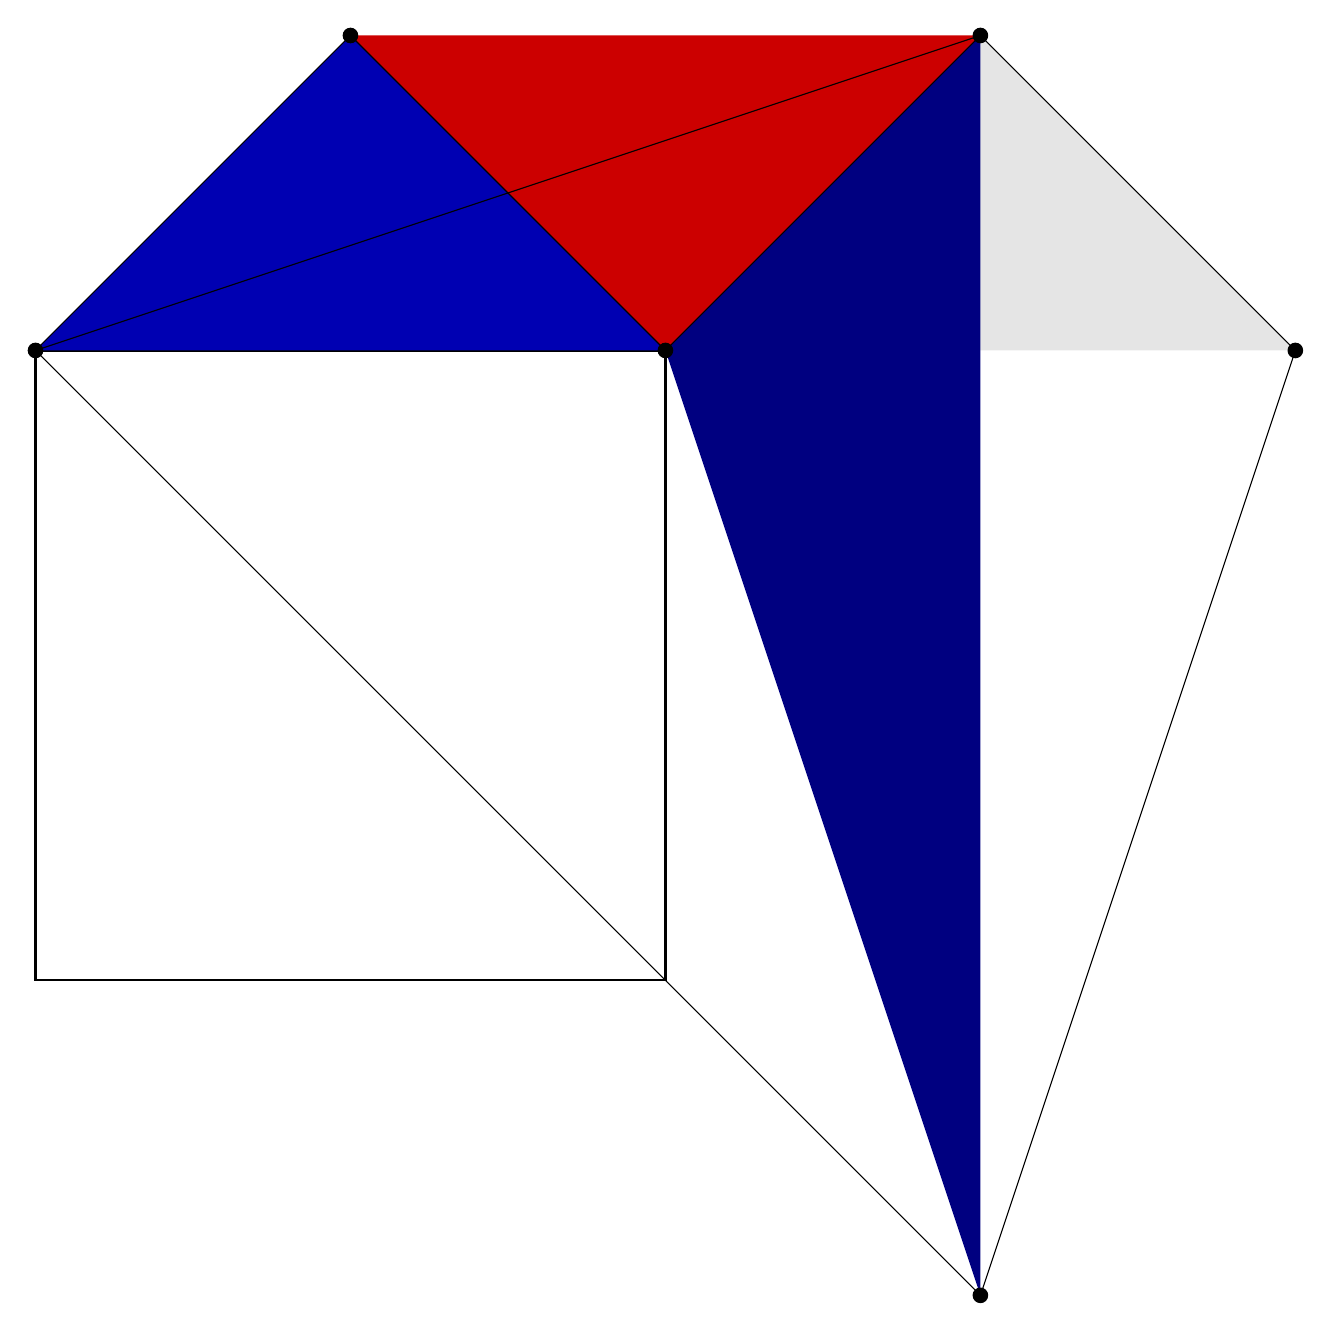
\begin{tikzpicture}[scale=2]

% Central square
\draw[thick] (0,0) rectangle (4,4);

% Triangles
\fill[blue!70!black] (0,4) -- (2,6) -- (4,4); % Top triangle
\fill[red!80!black] (2,6) -- (4,4) -- (6,6); % Right triangle
\fill[white!90!black] (4,4) -- (6,6) -- (8,4); % Bottom triangle
\fill[blue!50!black] (4,4) -- (6,6) -- (6,-2); % Left triangle

% Vertices
\node at (0,4) [circle, fill=black, inner sep=2pt] {};
\node at (2,6) [circle, fill=black, inner sep=2pt] {};
\node at (4,4) [circle, fill=black, inner sep=2pt] {};
\node at (6,6) [circle, fill=black, inner sep=2pt] {};
\node at (8,4) [circle, fill=black, inner sep=2pt] {};
\node at (6,-2) [circle, fill=black, inner sep=2pt] {};

% Edges
\draw (0,4) -- (2,6);
\draw (2,6) -- (4,4);
\draw (4,4) -- (6,6);
\draw (6,6) -- (8,4);
\draw (8,4) -- (6,-2);
\draw (6,-2) -- (0,4);
\draw (0,4) -- (6,6);

\end{tikzpicture}

\end{document}